\chapter {Resultados}
Foram analisados através de mais de 67.648.820 de \textbf{LOC} nos projetos Ant, Checkstyle, CommonsCollections,  FindBugs,  FreeMind,  Hibernate,  JBoss,  Jetty,  Log4j,  Spring,  SquirrelSql,  Weka,  Xerces.\\

\section{LambdaExpression}
A maior mudança ocorrida em Java 8 foi a introdução de expressões lambda, que tem por definição prover um bloco de código limpo e conciso para representar um interface usando uma simples expressão. Também melhoram a manipulação de \textit{collections} tornando fácil a iteração através de filtros para extração de dados e adiciona novas características de concorrência que aumenta a performance em ambientes \textit{multicores}.\\

\textit{Anonymous inner classes} foram projetada para facilitar o desenvolvedor a tratar seus dados de forma fácil, mas isso não é tão simples como deveria ser, além de suas implementações serem usadas somente em local específico da aplicação, em boa parte de seu uso para tratar eventos decorrentes do usuário ou de algum processamento específico. Expressões Lambda podem vir a substituir \textit{Anonymous inner classes} o que acarreta em uma redução na quantidade de linhas de código significativamente além de reduzir os tipos utilizados no sistema.\\

Dentre os projetos analisados foram encontrados ocorrências de tal característica, \textit{Lambda Expression}, somente nos projetos \textit{Checkstyle}, \textit{Hibernate}, \textit{Jetty} \textit{Spring}, totalizando 774 ocorrências dentre um total de 64.179.440 \textbf{LOC}.\\

Tendo em vista que expressões lambdas podem vir a substituir \textit{Anonymous inner classes} e \textit{Types} dos projetos segundo \cite{Java8Lambda}. Foram encontradas nos projetos \textit{CheckStyle}, \textit{Hibernate}, \textit{Jetty} e \textit{Spring}, 2201, 13654, 10016 e 113069 ocorrências respectivamente totalizando em 138940 ocorrências de \textit{Anonymous inner classes}. Com uso de expressões lambda a quantidade de ocorrências de \textit{Anonymous inner classes} e \textit{Types} teria a tendência natural de diminuir seu uso.\\

Um uso corriqueiro de expressão lambda seria para substituir o seguinte bloco do projeto Checkstyle:
\begin{lstlisting}
	//Without Lambda Lambda Expression
	button.addActionListener(new ActionListener(){
		public void actionPerformed(ActionEvent e) {
			System.out.println("button clicked");
		}
	});

	//With Lambda Lambda Expression
	button.addActionListener(event -> System.out.println("button clicked"));
	
	//###########################################################################
	
	TreeSet<String> paths = new TreeSet<String>(
			new Comparator<String>({
				public int compare(String o1, String o2){
					int paths1 = new StringTokenizer(o1,"/",false).countTokens();
					int paths2 = new StringTokenizer(o2,"/",false).countTokens();
				
					if (paths1 == paths2){
						return o1.compareTo(o2);
					}
				
					return paths2 - paths1;
				}
			}
	);
	
	
	ps = paths.stream().filter(p -> p.o1 != p.o2)
					   .collect(Collectors.toSet());
	
	return new TreeSet(ps);
	
\end{lstlisting}

Como este simples exemplo pode-se verificar do benefício das expressões lambda tendo em vista que  redução do uso de \textit{Anonymous inner classes} além de ser uma forma mais atual. Neste seria um redução de 80\% sobre o código utilizado anteriormente. Além da redução de tipos 3 tipos(\textit{ActionListener}, \textit{ActionEvent} e \textit{void}) para um único método anônimo que acarreta em 300\% na redução de tipos,  se fosse possível aplicar esta características em todas as 138940 ocorrências de \textit{Anonymous inner classes} seria uma redução significativa de \textbf{LOC}.

Entretanto diante dos dados coletados é possível afirmar que Expressões Lambda não estão sendo adotadas com este intuito, o que pode leva a crer que esta característica por ser recente ainda pode não ter sido bem acolhida pela comunidade de desenvolvedores para tirar proveito desta  característica para benefício de seus projetos.\\

\section{MultiCatch}
Com o advento do Java 7, foi introduzido o suporte a \textit{MultiCatch} que trouxe a possibilidade de trazer clareza e simplicidade ao código escrito.\\

De todos os projetos analisados foram encontradas na soma das ocorrências 5247 estruturas que usam esse artificio. Os projetos que tiveram mais ocorrências de \textit{multicatchs} foram \textit{FindBugs}, \textit{Ant}, \textit{Log4j}, \textit{Checkstyle}, 976, 3133, 252 e 434 respectivamente.\\

\section{ANT}
Até a última versão deste projeto, 1.9.5, não foram encontradas utilização métodos com \textit{vargs}, expressões lambdas, \textit{switch} com \textit{strings} e nem \textit{try} com \textit{resources}.\\

Este projeto faz um bom uso de tratamento de exceções sendo encontrado em toda história de desenvolvimento foram produzidas 28 versões deste e com um total de 34722 blocos \textit{trys}, onde em média foram encontradas 1240 destes blocos por versão. E deste total pode-se verificar um total de 513 ocorrências de blocos \textit{trys} com \textit{catchs} iguais totalizando em 1,5\% de código repetido neste quesito conforme ilustra Figura: \ref{fig:TrysAnt}.\\

	\begin{figure}[h]
		\center
		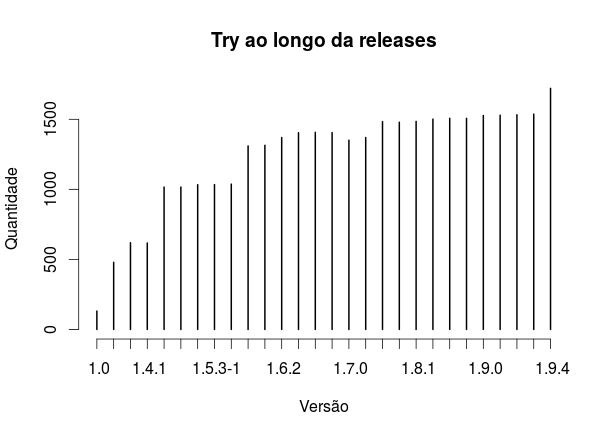
\includegraphics[width=0.7\textwidth]{Imagens/trysAnt}
		\label{fig:TrysAnt}
		\caption{Tratamento de exceção ao longo das releases.}
	\end{figure}

Entretanto pode-se constatar conforme ilustrado na Figura: \ref{fig:catchIguais} que em todas as versões do projeto \textit{ANT} possui o tratamento de exceção como blocos \textit{catchs} iguais sendo contabilizado um total de 513 ocorrências e dando atenção especial entre as versões 1.9.0 e 1.9.5. Entretanto a partir da versão 1.9.0 por volta de 2012, java possuía o mecanismo de \textit{multicatch} que fora lançado por volta de 2011 em java 7. Entre as \textit{releases} desta versão foram encontradas em cada um dos 5 lançamentos do \textit{ANT} por volta de 27 ocorrências iguais de \textit{catchs} e acarreta em um total de 135 blocos repetidos. Caso fosse adotado \textit{multicatch} seria reduzido somente a 5 blocos a cada versão existente o que seria uma redução de código repetido em aproximadamente 18\%, e isso acarretaria em um código mais atual e elegante.\\

	\begin{figure}[h]
		\center
		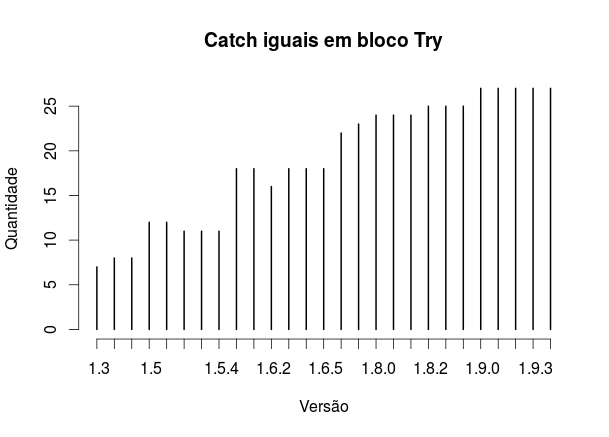
\includegraphics[width=0.7\textwidth]{Imagens/catchsIguais}
		\label{fig:catchIguais}
		\caption{Bloco Try com catchs iguais ao longo das releases.}
	\end{figure}
